\section{Technical summary}

% Brief summary of the approach used by the authors and their contributions

The authors approach retinal vessels and optic disc segmentation as an image-to-image regression task by designing a novel CNN architecture derived from the VGG network \cite{simonyan_very_2014}. They adapt the final layers of the base network and use the coarser ones to generate the optic disc segmentation and the finer ones for the vessels. This report focuses only on the vascular segmentation. Figure \ref{fig:driu} shows an overview of the designed architecture.

\begin{figure}[H]
  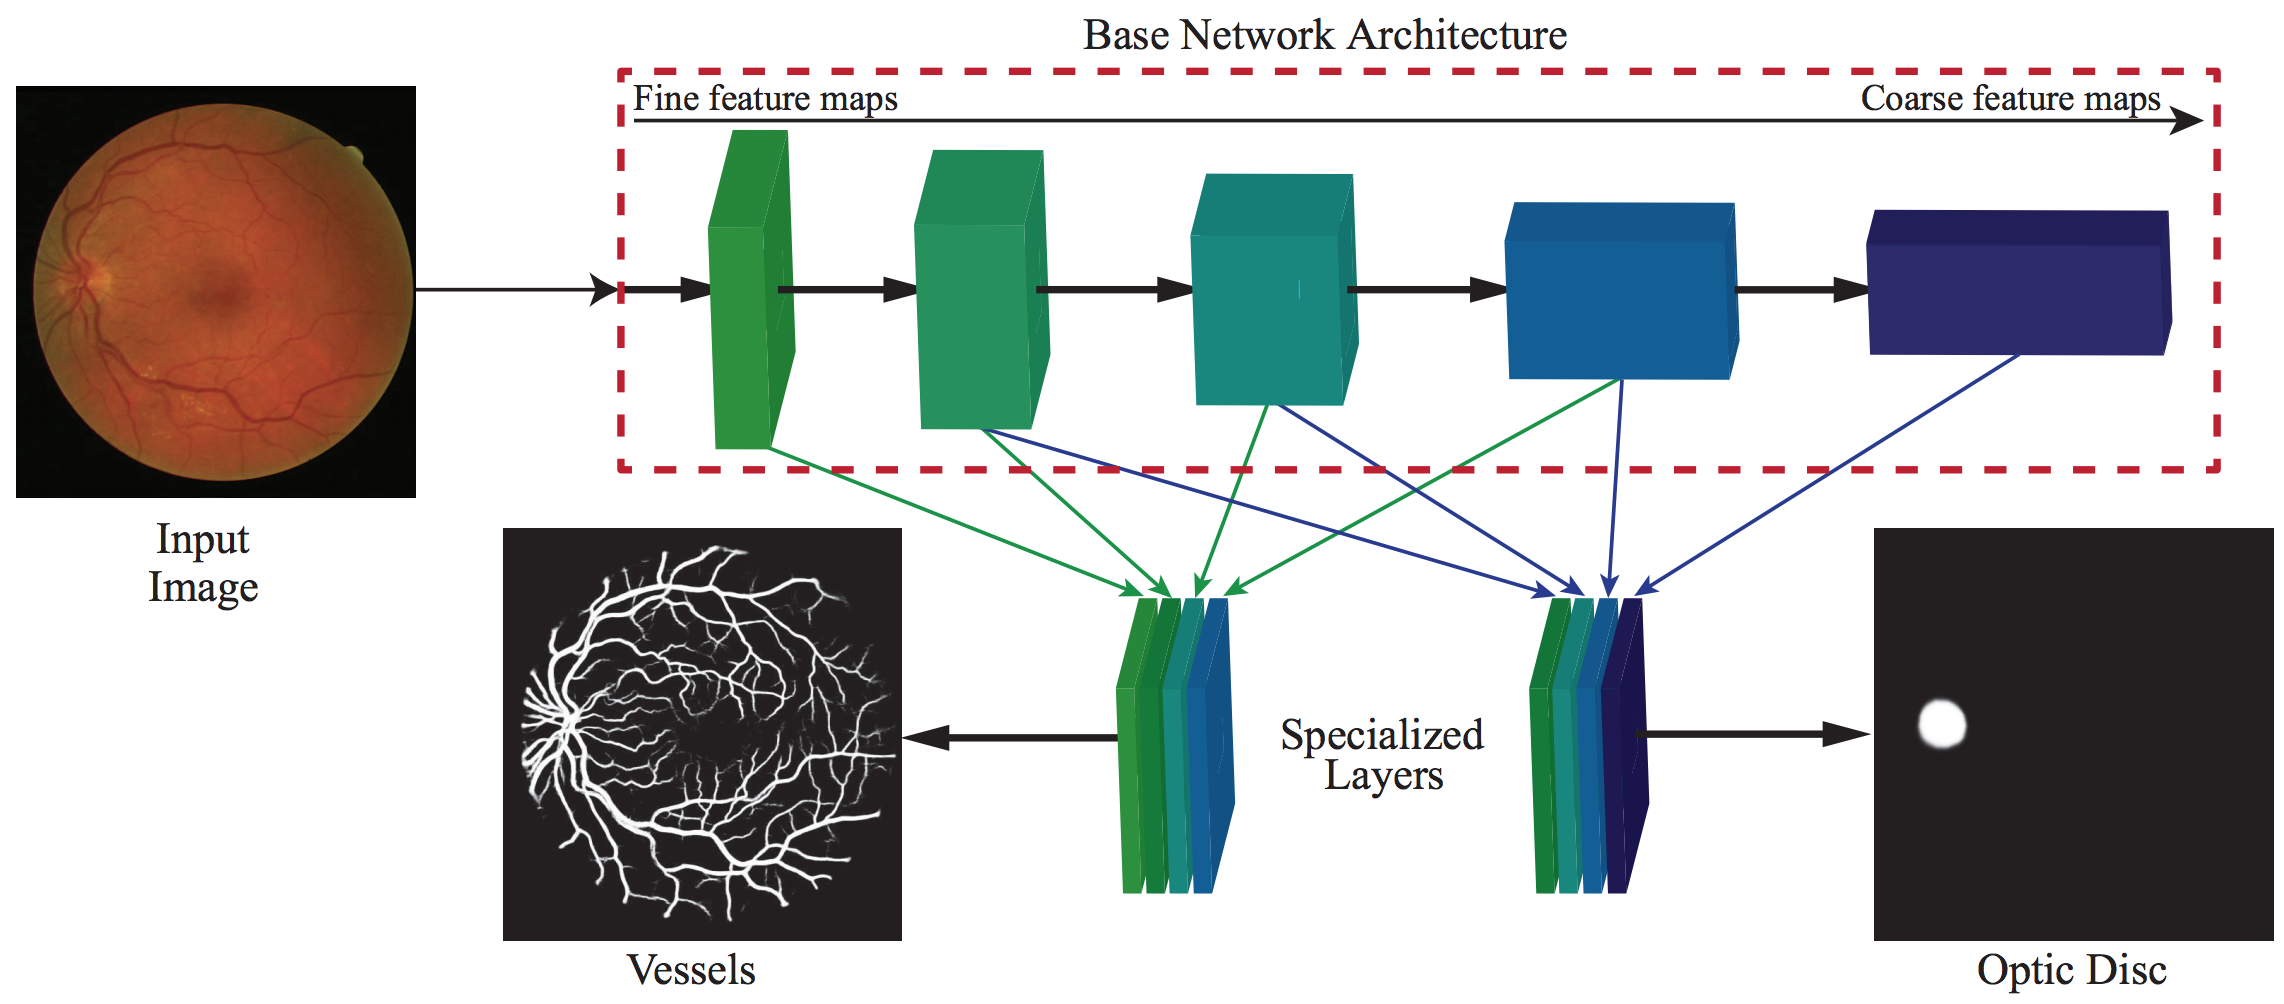
\includegraphics[width=\textwidth]{figures/driu}
  \caption{Overview of the architecture designed for DRIU \cite{maninis_deep_2016}.} \label{fig:driu}
\end{figure}

The loss function used for training is a class-balancing cross entropy given the severely biased ground truth, where approximately 10 \% of the pixels are vessels, while the rest represent background. The weight $\beta$ used to handle the imbalance is set to $\beta = |Y_-| / |Y|$, where $Y$ is the ground truth (first annotator) label image and $Y_-$ is the set of background pixels in $Y$. The probability $P(.)$ obtained in the regressed output map is obtained by applying a sigmoid $\sigma(.)$ to the activation of the final corresponding convolutional layer.

The authors claim that their method is orders of magnitude faster than the state of the art. Their method is more accurate since the area under the precision-recall curve is the largest of all compared methods. They also claim to have reached super-human consistency (higher Dice score than second annotator with respect to the ground truth) and accuracy (their method detects small vessels that seem to have been missed by the annotators).
